\section{Software requirements}

To program the PSoC microcontroller, you need to install the PSoC Creator software suite. You can download this software on the following website: \\
\url{https://www.cypress.com/products/psoc-creator-integrated-design-environment-ide}. The software is quite large, so it might take a while to download. You can then install the software suite. \\
You should also download the CY8CKIT-059 Kit setup on \url{https://www.cypress.com/file/416376/download} (you might need to create an account to download this file). Once downloaded, you should execute the downloaded file to install the CY8CKIT-059 Kit.
\\
\\
When launching the PSoC Creator IDE, it will usually ask you to register. You can ignore this by selecting ``Register later''. When creating a new project, you need to specify which microcontroller you are using. In this project, we will use the ``CY8CKIT-059 (PSoC 5LP)''. Once your project is created, your project will be loaded as shown in Figure~\ref{fig:psoc_creator_ide}. 
\begin{figure}[h]
	\centering
	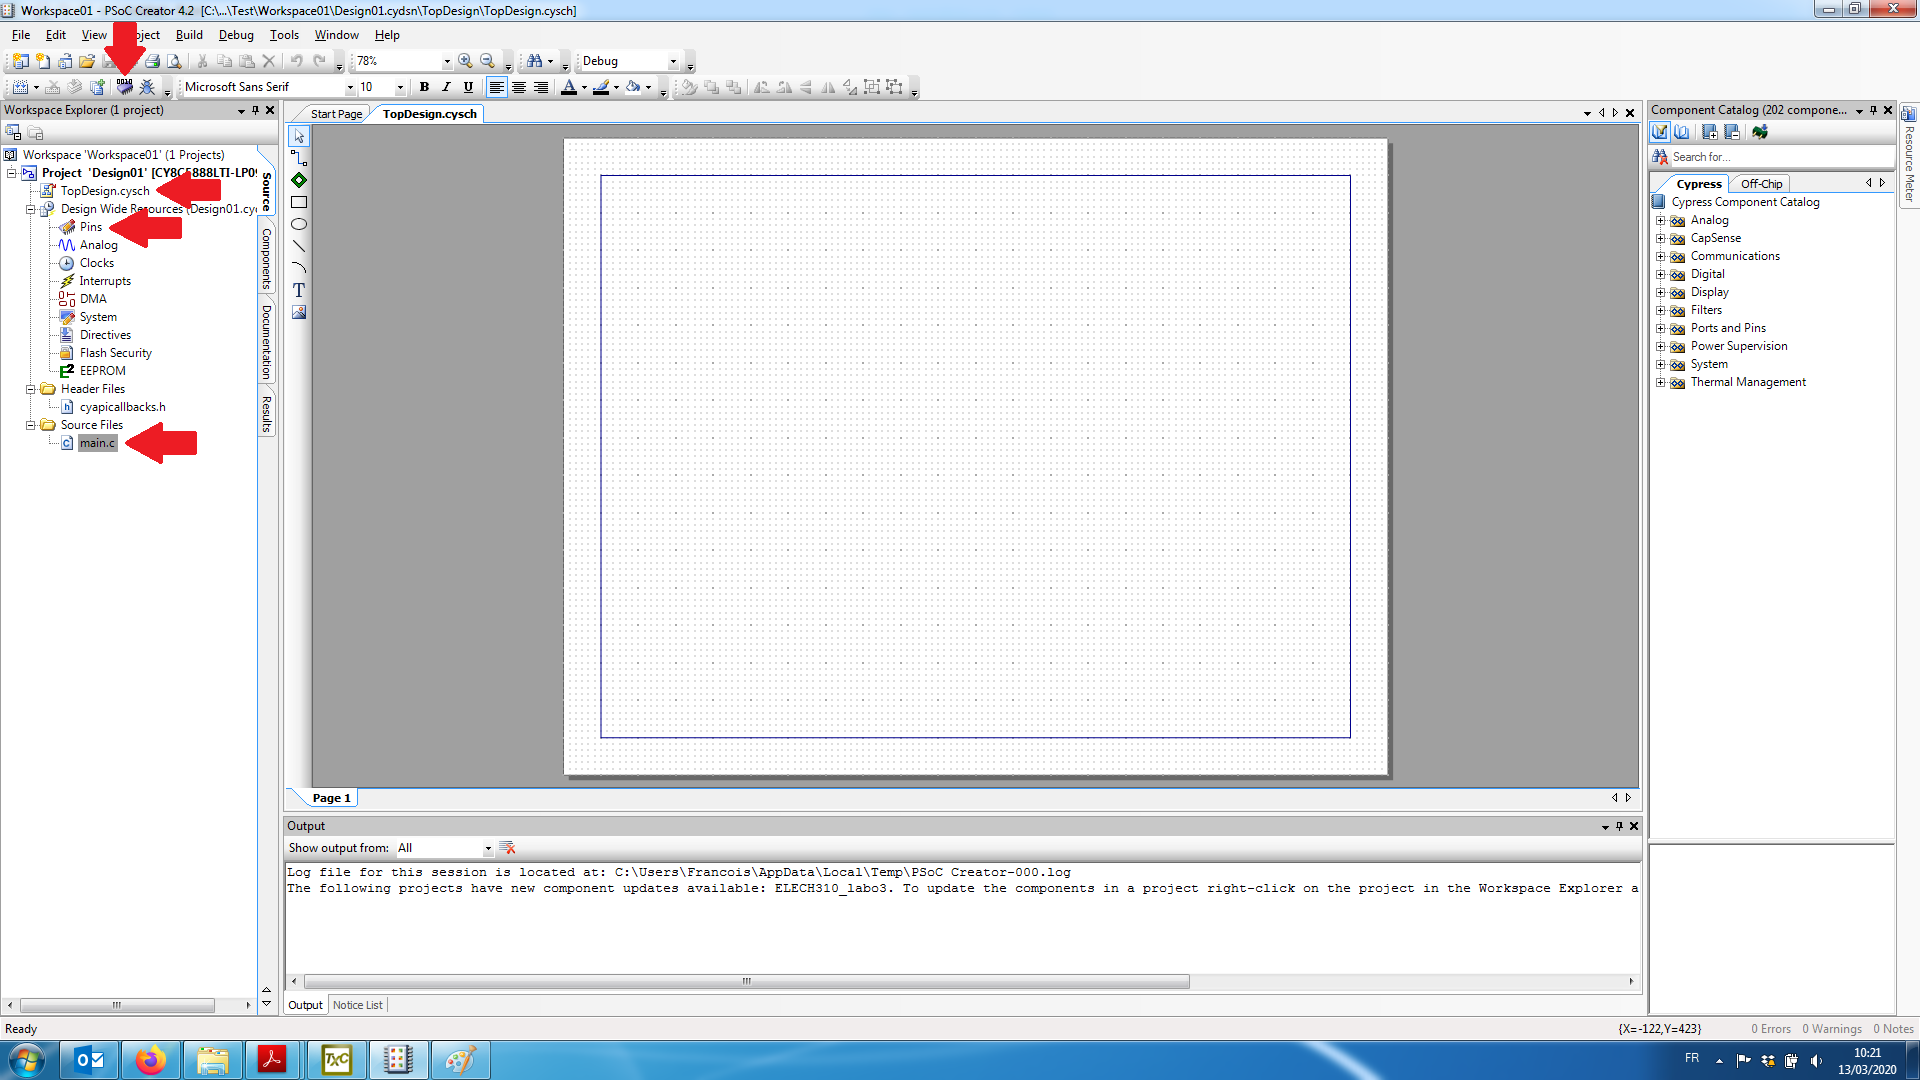
\includegraphics[width=5in]{psoc_creator_ide.png}
	\caption{PSoC Creater IDE. }
	\label{fig:psoc_creator_ide}
\end{figure}
\begin{figure}[h]
	\centering
	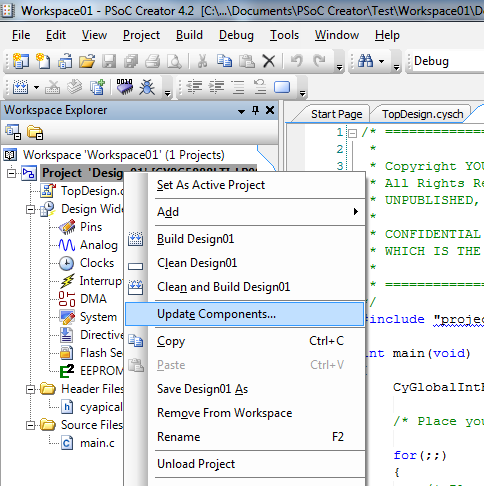
\includegraphics[width=2in]{update_components.png}
	\caption{How to update the PSoC firmware. }
	\label{fig:update_components}
\end{figure}

In this project, you will mainly be using three tabs of the IDE: 
\begin{itemize}
	\item \textbf{TopDesign.cysch: } In this window, you will instantiate all the hardware elements that you will use in the microcontroller, i.e. the GPIOs, the ADC, the DAC, the PWM, the LCD screen, etc. 
	\item \textbf{Pins: } This window will help you to associate each hardware element you instantiated to an actual output pin of the PSoC board. The numbers of each pin is written on the PSoC board itself, and you can use the document \texttt{Extension\_PSoC.pdf} to see which pin of the PSoC board was connected to which input/output of the custom-designed extension board. One of the particularities of the PSoC board is that each hardware element can be connected to any pin. 
	\item \textbf{main.c: } In this window you will write the firmware, i.e. the actual program that will be executed on the microcontroller. The code mainly consists of a main function that contains an initialization code and an infinite for-loop. Your microcontroller will continuously execute the program that is written in the infinite for-loop until the microcontroller is turned off.  
\end{itemize}

To upload your program to the PSoC board, connect the PSoC programmer to your computer with the USB cable, and click the ``Program'' button. This will build, compile and upload your project to the microcontroller. Useful documentation can be found on the following websites: 
\begin{itemize}
	\item Getting Started with PSoC 5LP: \url{https://www.cypress.com/file/41436/download}
	\item Tutorials for each hardware element of the PSoC: \url{www.cypress.com/psoc101}
  \item Video example on how to use the PSoC: \url{https://www.cypress.com/video-library/PSoC}
\end{itemize}
It is possible that the first time you try to upload a program to the PSoC board, you get an error message. This is because the firmware on the PSoC board needs to match the software version of PSoC Creator IDE. To solve this problem, right-click on the project and select ``Update components'' (see Figure~\ref{fig:update_components}. Then just follow the instructions with the default settings. 
